% KDD submissions use the ACM proceedings template.
% For camera-ready, remove the anonymous/review options and fill in the
% official conference metadata, rights, DOI, ISBN, and author blocks.
\PassOptionsToPackage{table}{xcolor}
\documentclass[sigconf,anonymous,review]{acmart}
\citestyle{acmnumeric}
\setcopyright{none}
\settopmatter{printacmref=false, printccs=false, printfolios=true}
\renewcommand\footnotetextcopyrightpermission[1]{}
\acmConference[KDD '26]{Proceedings of the ACM SIGKDD Conference on Knowledge Discovery and Data Mining}{August 2026}{Korea}
\acmBooktitle{Proceedings of the ACM SIGKDD Conference on Knowledge Discovery and Data Mining (KDD '26), August 2026, Korea}
\acmYear{2026}
\copyrightyear{2026}
\acmDOI{}
\acmISBN{}
\acmSubmissionID{TODO}
\usepackage[T1]{fontenc}
\usepackage{booktabs}
\usepackage{amsmath}
\usepackage{amssymb}
\usepackage{amsfonts}
\usepackage{nicefrac}
\usepackage{array}
\usepackage{multirow}
\usepackage{makecell}
\usepackage{colortbl}
\usepackage{xspace}
\usepackage{tabularx}
\usepackage{algorithm}
\usepackage{algpseudocode}
\usepackage[capitalize]{cleveref}
\setcitestyle{numbers,square,comma,sort&compress}
\graphicspath{{./}{appendix_image/}}
\crefname{section}{Sec.}{Secs.}
\Crefname{section}{Section}{Sections}
\crefname{table}{Tab.}{Tabs.}
\Crefname{table}{Table}{Tables}
\crefname{figure}{Fig.}{Figs.}
\Crefname{figure}{Figure}{Figures}
\crefname{equation}{Eq.}{Eqs.}
\Crefname{equation}{Equation}{Equations}
\setcounter{topnumber}{5}
\setcounter{bottomnumber}{5}
\setcounter{totalnumber}{10}
\renewcommand{\topfraction}{0.95}
\renewcommand{\bottomfraction}{0.95}
\renewcommand{\textfraction}{0.05}
\renewcommand{\floatpagefraction}{0.8}
\renewcommand{\dbltopfraction}{0.95}
\renewcommand{\dblfloatpagefraction}{0.8}
\setlength{\textfloatsep}{10pt plus 2pt minus 2pt}
\setlength{\floatsep}{8pt plus 2pt minus 2pt}
\setlength{\intextsep}{10pt plus 2pt minus 2pt}
% Paper macros.
\newcommand{\methodname}{\textsc{Spine}\xspace}
\newcommand{\ppp}{\textsc{PPP}\xspace}
\newcommand{\redadd}[1]{\textcolor{red}{#1}}
\newcommand{\redfill}[1]{\textcolor{red}{\textbf{[#1]}}}
\newcommand{\softpara}{\vspace{0.25em}}
\newcommand{\pmv}[2]{\ensuremath{#1\,{\scriptstyle\pm\,#2}}}
\title{\methodname{}: Single-Cell Perturbation-Field Inference in Niche Environments}
\author{Anonymous Author(s)}
\affiliation{%
  \institution{Anonymous Institution}
  \city{Anonymous}
  \country{Anonymous}
}
\email{anonymous@example.com}
\raggedbottom
\begin{document}
\maketitle
\begin{abstract}
Genetic and drug perturbation models are increasingly used to predict cellular responses to interventions, but most are learned from dissociated single-cell assays and therefore miss how perturbation effects propagate through intact tissue. We formulate spatial perturbation prediction as a two-stage problem: first identifying direct-effect cells and estimating their cell-intrinsic transcriptional changes from observed perturbation data or a single-cell perturbation model such as CPA, and then predicting how these direct effects reshape neighboring cells in the tissue graph. \methodname{} addresses the second stage by predicting a perturbation-induced response field from an unperturbed tissue graph and a direct-effect seed. Because cell-resolved supervision for spatial propagation is scarce, we construct an audited Pre-Post Perturbation (PPP) benchmark from matched Spatial Perturb-seq control--perturbation pairs. \methodname{} is a perturbation-aware graph neural network that decomposes each cell's response into niche impact and direct-effect-to-neighbor propagation impact. A masked niche branch estimates the microenvironment-explainable component, a propagation branch routes direct-effect seeds through the local tissue graph, an ST-pretrained niche encoder provides microenvironment priors from large-scale spatial transcriptomics, and a distance-aware refinement module jointly refines the final response field. We validate \methodname{} on cell-resolved Spatial Perturb-seq, synthetic ligand--receptor propagation, and real Perturb-map benchmarks.Across these settings, \methodname{} outperforms statistical, retrieval, diffusion, fixed-communication, linear, and generic graph baselines, achieving 0.684/0.457 neighbor/ring Pearson on block-held-out Spatial Perturb-seq, 0.596/0.451 in grouped guide-out validation, and up to 0.853 spot-level program agreement in Perturb-map. Ablations confirm the importance of direct-effect seeds, edge features, and niche--propagation decomposition. A de novo IFN-$\gamma$ case study further illustrates how \methodname{} can combine an unperturbed tissue section with an external direct-effect seed to generate spatial response-field hypotheses.
\end{abstract}
% Predicting how genetic perturbations reshape transcriptional states within native tissue is central to mapping cell-fate decisions in development, decoding tissue dysregulation in disease, and guiding cell-type- and niche-specific target prioritization~\citep{dixit2016perturbseq,norman2019combinatorial,zheng2024invivo,finan2017druggable,king2019genetic}. 
% However, most perturbation data come from dissociated tissue, removing the cell--cell signaling and niche architecture that govern perturbation responses in vivo~\citep{adamson2016crispr,datlinger2017cropsseq,replogle2022mapping,frangieh2021multimodal}. 
% Spatial functional genomics, including Perturb-map, Perturb-FISH, and Spatial Perturb-Seq, begins to close this gap by placing CRISPR perturbations within intact tissue and reading out molecular state in situ~\citep{dhainaut2022spatialcrispr,binan2025perturbfish,shen2026spatialperturbseq}. 
% These measurements shift the modeling problem from predicting isolated cell-intrinsic responses to predicting how perturbation effects propagate through spatially organized tissue. 
% Without models that infer sender-to-receiver responses under local communication and geometry, spatial Perturb-Seq remains difficult to translate into predictive target prioritization.
\section{Introduction}
Predicting genetic-perturbation responses in native tissue is central to mapping development and prioritizing niche-specific therapeutic targets~\citep{dixit2016perturbseq,norman2019combinatorial,zheng2024invivo,finan2017druggable,king2019genetic}. Most data come from dissociated Perturb-seq and pooled CRISPR assays, which support cell-intrinsic modeling but remove the cell--cell communication and niche architecture that shape many in vivo effects~\citep{adamson2016crispr,datlinger2017cropsseq,replogle2022mapping,frangieh2021multimodal}. Spatial functional genomics assays, including Perturb-map, Perturb-FISH, and Spatial Perturb-Seq, restore this tissue layer by placing perturbations in intact tissue and reading out molecular state in situ~\citep{dhainaut2022spatialcrispr,binan2025perturbfish,shen2026spatialperturbseq}. They shift the target from isolated cell responses to spatial response fields, but remain too costly to cover perturbation--context combinations exhaustively.
Existing methods cover only fragments of this problem. Single-cell perturbation-response models use latent translation, optimal transport, gene-relation graphs, disentangled representations, or foundation models~\citep{lotfollahi2019scgen,bunne2023cellot,roohani2023gears,piran2024biolord,theodoris2023geneformer,cui2024scgpt,hao2024scfoundation}, but lack a tissue graph for propagation. Spatial transcriptomics and communication methods preserve geometry, niches, and plausible cell--cell routes~\citep{stahl2016spatial,vickovic2019hdst,rodriques2019slideseq,stickels2021slideseqv2,cang2023commot,dries2021giotto,phan2023stlearn,tiling2024nicheformer}, but do not predict which perturbation activates which route or the signed magnitude of neighbor responses. The missing interface maps direct effects onto neighbors in an intact tissue graph.
We formulate spatial perturbation prediction as two stages. Given an ST slide and a perturbation, one first locates direct-effect cells and estimates their cell-intrinsic transcriptional changes. Direct-effect cells can be specified by guide labels, experimental design, or manual intervention sites; their direct-effect profile can be measured or predicted by a fine-tuned single-cell perturbation model such as CPA~\citep{Lotfollahi2023}. \methodname{} addresses the second stage: conditioned on the tissue graph and direct-effect seed, it predicts neighbor changes.
This setting presents three challenges. \textbf{Challenge 1.} Spatial perturbation data are scarce, limiting direct supervision for propagation. We build Pre--Post Perturbation Pairing (PPP) from Spatial Perturb-Seq~\cite{shen2026spatialperturbseq}: each perturbed post patch is paired with matched control-like pre-state patches, forming pairs with estimated initial states and response targets. Together with a controlled synthetic LR benchmark built from GSE157977 mouse in vivo Perturb-seq profiles and NicheNet v2 mouse ligand--target priors~\citep{jin2020invivo,browaeys2020nichenet,browaeys2022nichenetv2}, plus Perturb-map/GSE193460 validation~\citep{dhainaut2022spatialcrispr}, PPP provides cell-resolved supervision, rule-controlled tests, and coarser real spatial readout agreement.\textbf{Challenge 2.} Neighbor responses mix perturbation-driven propagation with endogenous microenvironment effects. \methodname{} uses a niche--propagation architecture: the niche module masks perturbation inputs to estimate niche impact from baseline expression, cell-state composition, spatial geometry, and local context, while the propagation module routes direct-effect seeds through the tissue graph to predict remaining propagation impact. Distance-aware refinement integrates signals across radial neighborhoods. \textbf{Challenge 3.} Spatial perturbation models must generalize beyond measured perturbation--context pairs. We mine response-like microenvironments from unperturbed mouse-brain ST: two HD sections and three Xenium studies, totaling $392{,}962$ cells. Seven templates spanning interferon/inflammatory, microglial, astrocytic, myelin-lineage, neuronal, splicing, and mitochondrial/OXPHOS programs yield $1{,}619$ positive anchors and $9{,}316$ anchor--normal local pairs. These pairs pretrain a reference-ST niche encoder on gene programs, neighborhood structure, patch composition, and communication plausibility without perturbation labels.
Across three validation settings, \methodname{} shows consistent performance. On block-held-out mouse-brain Spatial Perturb-Seq, it outperforms statistical, retrieval, diffusion, fixed-CCC, linear, and generic graph baselines, reaching neighbor/ring Pearson $0.684/0.457$ with lower Neighbor MAE. Under a stricter grouped guide-out split, we jointly held out three unseen perturbation guides (\textit{fasn}, \textit{stk39}, and \textit{trem2}) and evaluated them separately; \methodname{} achieved stable per-guide neighbor Pearson values around $0.60$ and ring Pearson values around $0.45$, indicating that guide-out generalization was not driven by a single held-out guide. On synthetic LR propagation, it recovers known response fields with $0.619/0.815$ neighbor/ring Pearson; on external spot/lesion-level Perturb-map validation, it reaches spot-level program agreement up to Pearson $0.853$. Ablations support the design: removing niche-impact residualization causes the largest collapse to $0.165/0.153$, while removing edge features or direct-effect inputs also weakens performance.
\paragraph{Contributions.}
\begin{itemize}
    \item \textbf{An audited PPP benchmark for spatial perturbation propagation.} 
    We construct Pre--Post Perturbation Pairing (PPP) from Spatial Perturb-Seq to form matched pre-state and post-perturbation pairs with targets audited by multi-control stability, guide-specific nulls, shuffled-response controls, and leakage checks.
    \item \textbf{A niche--propagation model for direct-effect-to-neighbor prediction.} 
    \methodname{} decomposes each response into niche and propagation impact: a masked niche module captures microenvironment-explainable variation, a propagation module routes direct-effect seeds, and distance-aware refinement integrates radial signals.
    \item \textbf{Reference-ST perturbation-like priors without perturbation labels.} 
    We mine $392{,}962$ unperturbed mouse-brain ST cells to obtain $1{,}619$ positive anchors and $9{,}316$ anchor--normal pairs for reference-ST niche encoder pretraining.
    \item \textbf{A de novo tissue perturbation inference interface.} 
    \methodname{} combines a new ST tissue block with an external direct-effect seed to predict unmeasured spatial response fields, illustrated with an IFN-$\gamma$ mouse-brain case study.
\end{itemize}
\section{Related Work}
% \textbf{Spatial transcriptomics and spatial functional genomics.}
% Spatial transcriptomics enables gene-expression profiling with tissue coordinates, and recent high-resolution platforms and atlas-informed mapping methods improve cell-state interpretation in situ \citep{Stahl2016,Rodriques2019,Rao2021,Kleshchevnikov2022}. Spatial functional genomics further couples perturbations with intact-tissue readouts, making it possible to observe local and distal perturbation effects within native microenvironments \citep{Shen2026}. \methodname{} addresses the complementary prediction problem: given measured or predicted direct effects in sender cells, it predicts how responses propagate to spatial receivers.
\textbf{Spatial functional genomics assays.}
Spatial functional genomics couples pooled interventions with intact-tissue molecular
readouts. Perturb-map~\citep{dhainaut2022spatialcrispr} and
Perturb-FISH~\citep{binan2025perturbfish} map CRISPR perturbations with multiplexed
protein or RNA imaging, while Spatial Perturb-seq~\citep{shen2026spatialperturbseq}
extends this setting to transcriptome-wide in situ readout. These assays reveal
context-shaped perturbation effects, but remain sparse across perturbations,
cell types, neighborhoods, and tissue states, motivating models that generalize
spatial response fields beyond measured perturbation--context pairs.
\textbf{Single-cell perturbation modeling.}
Dissociated perturbation assays provide the main supervision for cell-intrinsic
response prediction, including Perturb-seq and CROP-seq
\citep{dixit2016perturbseq,adamson2016crispr,datlinger2017cropsseq}, combinatorial
and direct-capture Perturb-seq
\citep{norman2019combinatorial,replogle2020directcapture,replogle2022mapping},
Perturb-CITE-seq~\citep{frangieh2021multimodal}, and chemical-perturbation
benchmarks such as sci-Plex and OP3~\citep{srivatsan2020massively,szalata2024op3}.
Models built on these resources include conditional generative methods
\citep{lotfollahi2019scgen,lotfollahi2020trvae,Lotfollahi2023,hetzel2022chemcpa,kana2023scvidr,yu2025perturbnet},
optimal-transport and graph-based methods \citep{bunne2023cellot,roohani2023gears},
disentangled representation learning~\citep{piran2024biolord}, and foundation
models \citep{theodoris2023geneformer,cui2024scgpt,hao2024scfoundation}. These
methods provide useful direct-effect priors, but they operate on dissociated cells
and do not model direct-effect-to-neighbor propagation through local tissue graphs.
\textbf{Spatial tissue perturbation prediction.}
Recent tissue-level methods begin to connect perturbations with spatial context.
SpatialProp~\citep{spatialprop2025} propagates perturbation effects over spatial
graphs, Celcomen~\citep{celcomen2026} separates intra- and intercellular regulation
with causal generative modeling, and CONCERT~\citep{concert2025} predicts
niche-aware spot-level responses. \methodname{} is complementary: it predicts
cell-resolved direct-effect-to-neighbor response fields and validates them across
Spatial Perturb-seq, controlled synthetic LR propagation, and Perturb-map.
\begin{figure*}[t]
\centering
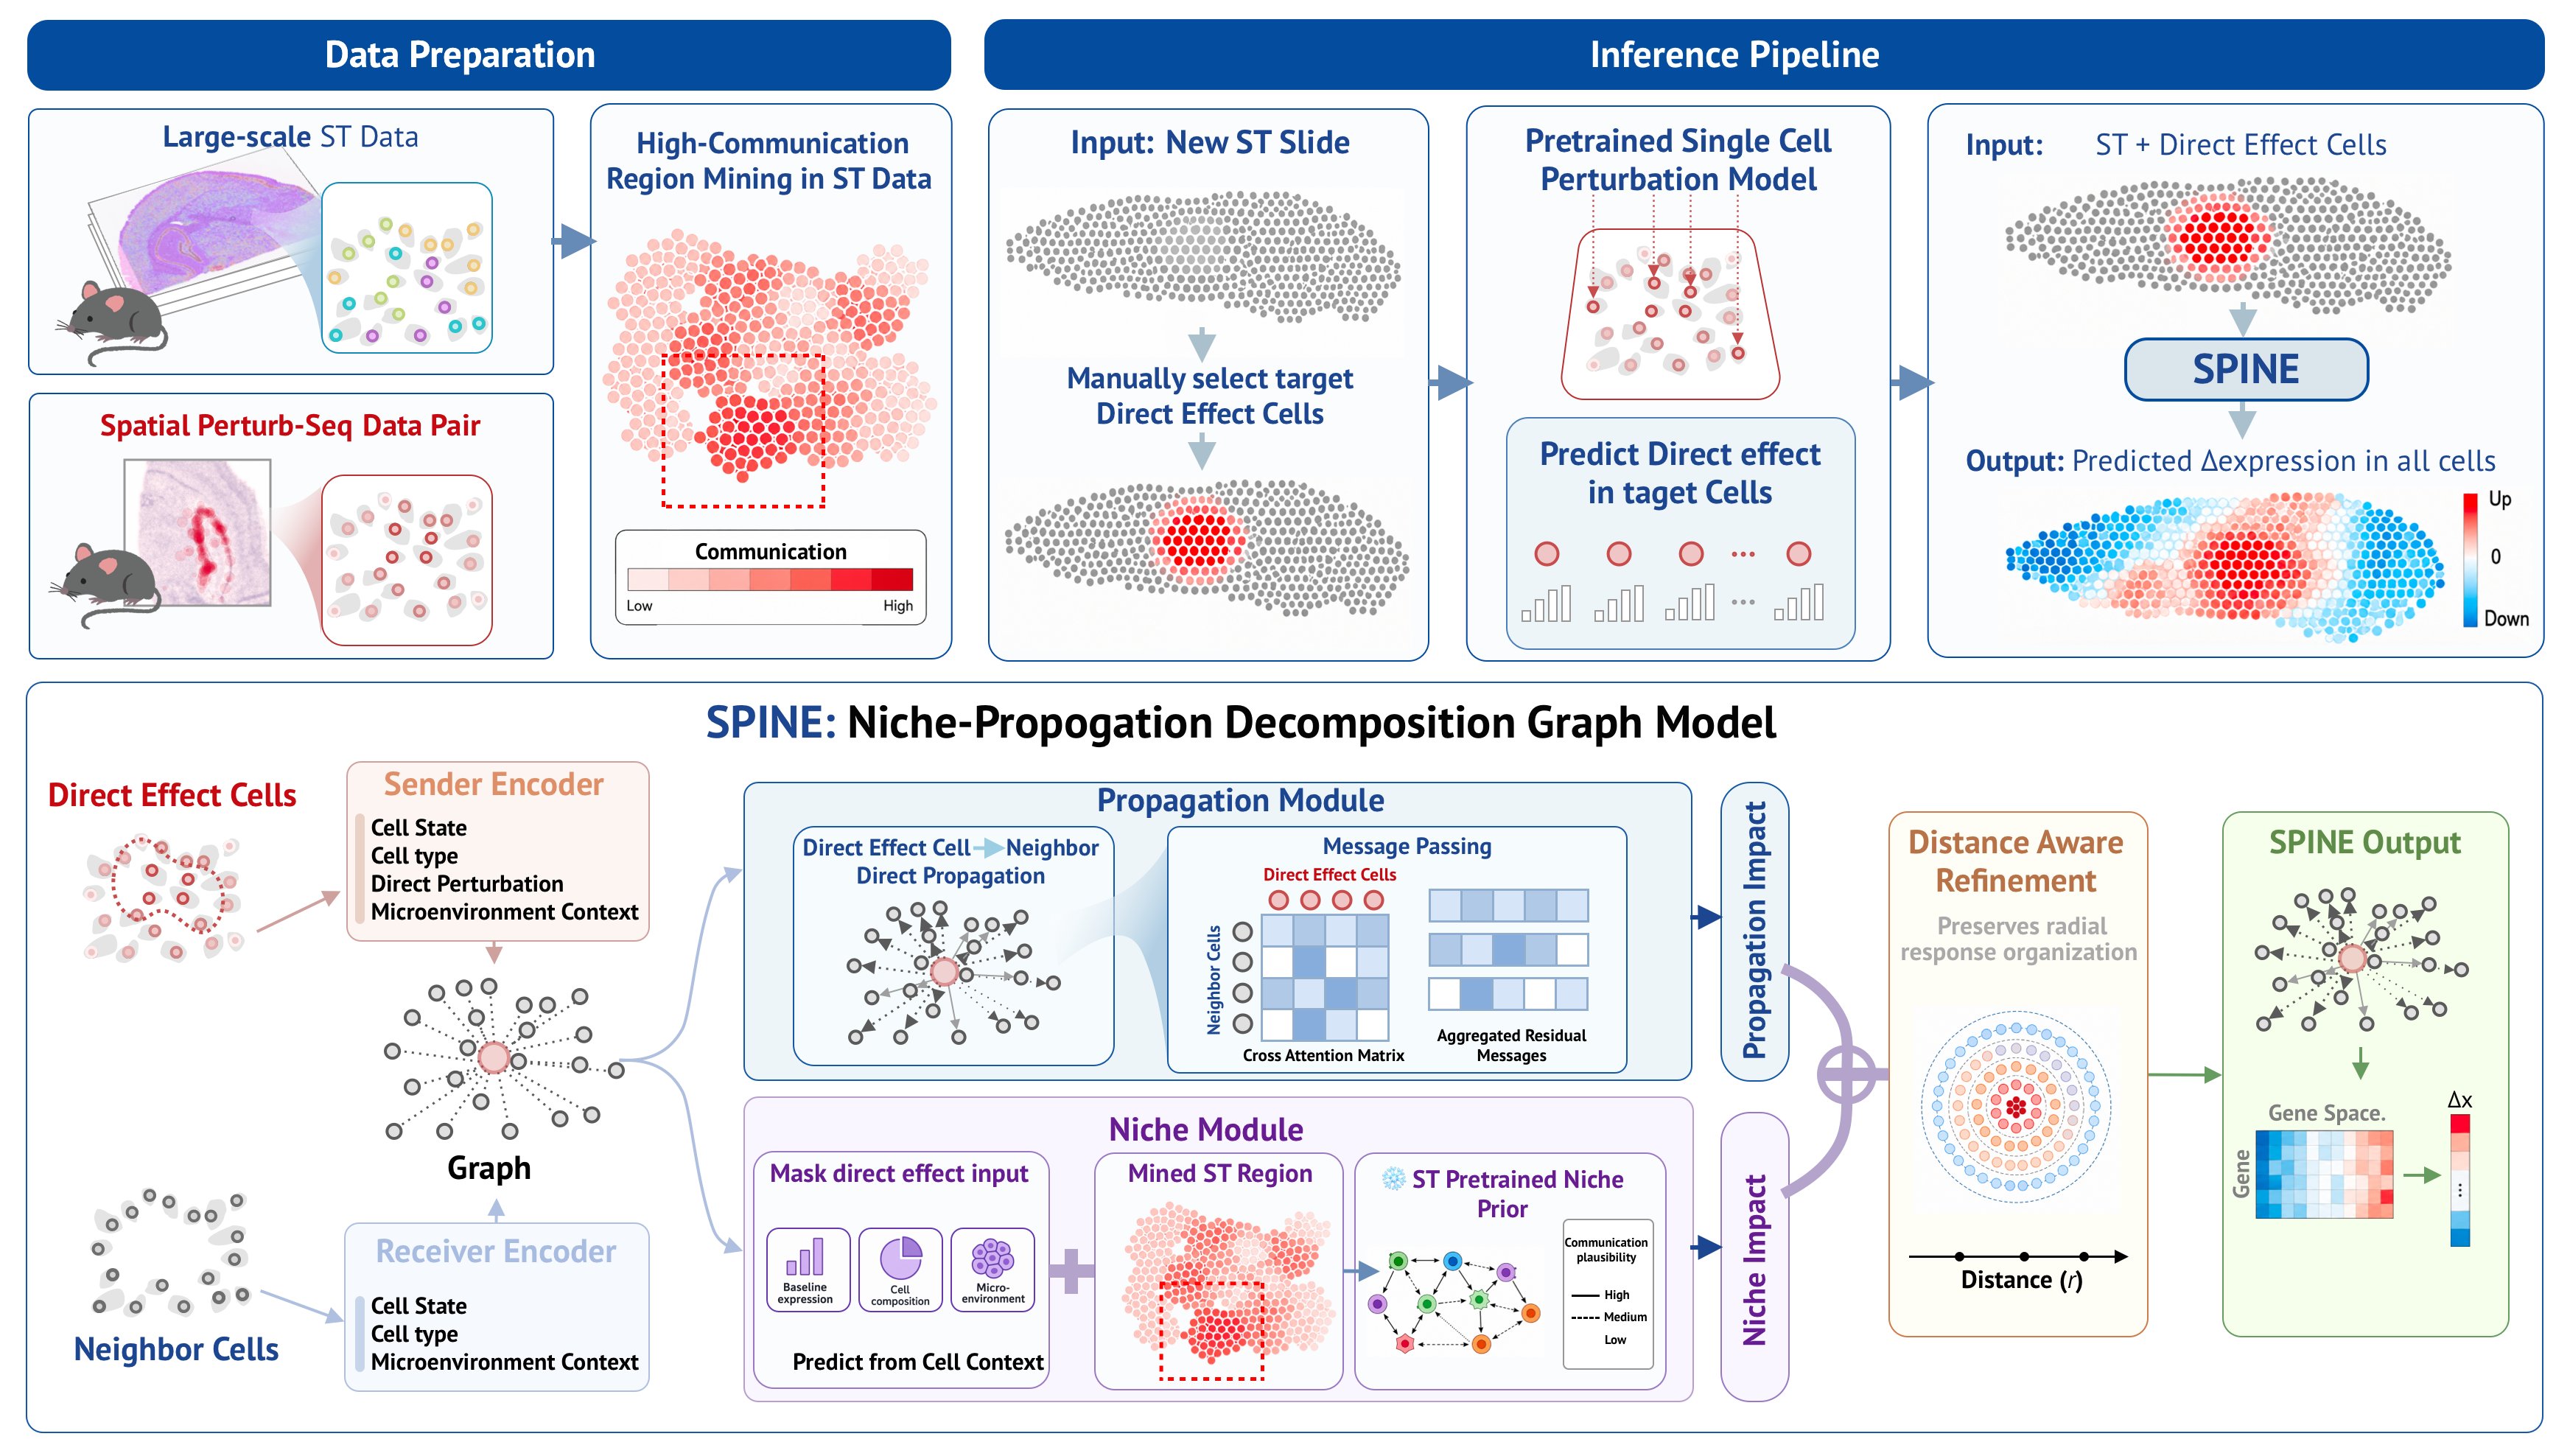
\includegraphics[width=0.98\linewidth]{model.png}
\caption{Overview of \methodname.}
\label{fig:main_framework}
\end{figure*}
\section{Data Preparation}
\label{sec:data_construction}
\subsection{Pre--Post Perturbation Pairing (PPP) Construction}
For each guide-positive anchor $a$, we form a 64-cell post-perturbation patch $P(a)=\{a\}\cup\mathcal{N}_{63}(a)$. Because the same cells are not observed before and after perturbation, we approximate the pre-perturbation state by matching the full post-perturbation patch, rather than only the guide-positive cell, to non-perturbed or control-like patches. We call this construction \textbf{Pre--Post Perturbation Pairing} (PPP). Candidate controls are ranked by spatial proximity, center-cell expression similarity, patch-level expression similarity, and cell-type composition; the top $K=3$ matches are softly aligned and aggregated into a consensus post-minus-matched-pre response target. \textbf{PPP target audit.}
PPP is a perturbation-consistent pseudo-target rather than directly observed causal ground truth. We therefore partition post anchors and candidate controls before matching, perform matching only within the same split, and ensure that no post anchor, matched-control anchor, or 64-cell control patch is shared across train/test partitions. Candidate pre-states use only non-perturbed or control-like cells, and model predictions are never used to construct targets. PPP responses show multi-control stability, recover expected gene-direction trends, and align better with own-guide signatures than with wrong-guide or target-shuffled nulls (Figure~\ref{fig:data_pair}). Details are provided in the supplementary material.
\begin{figure}[t]
\centering
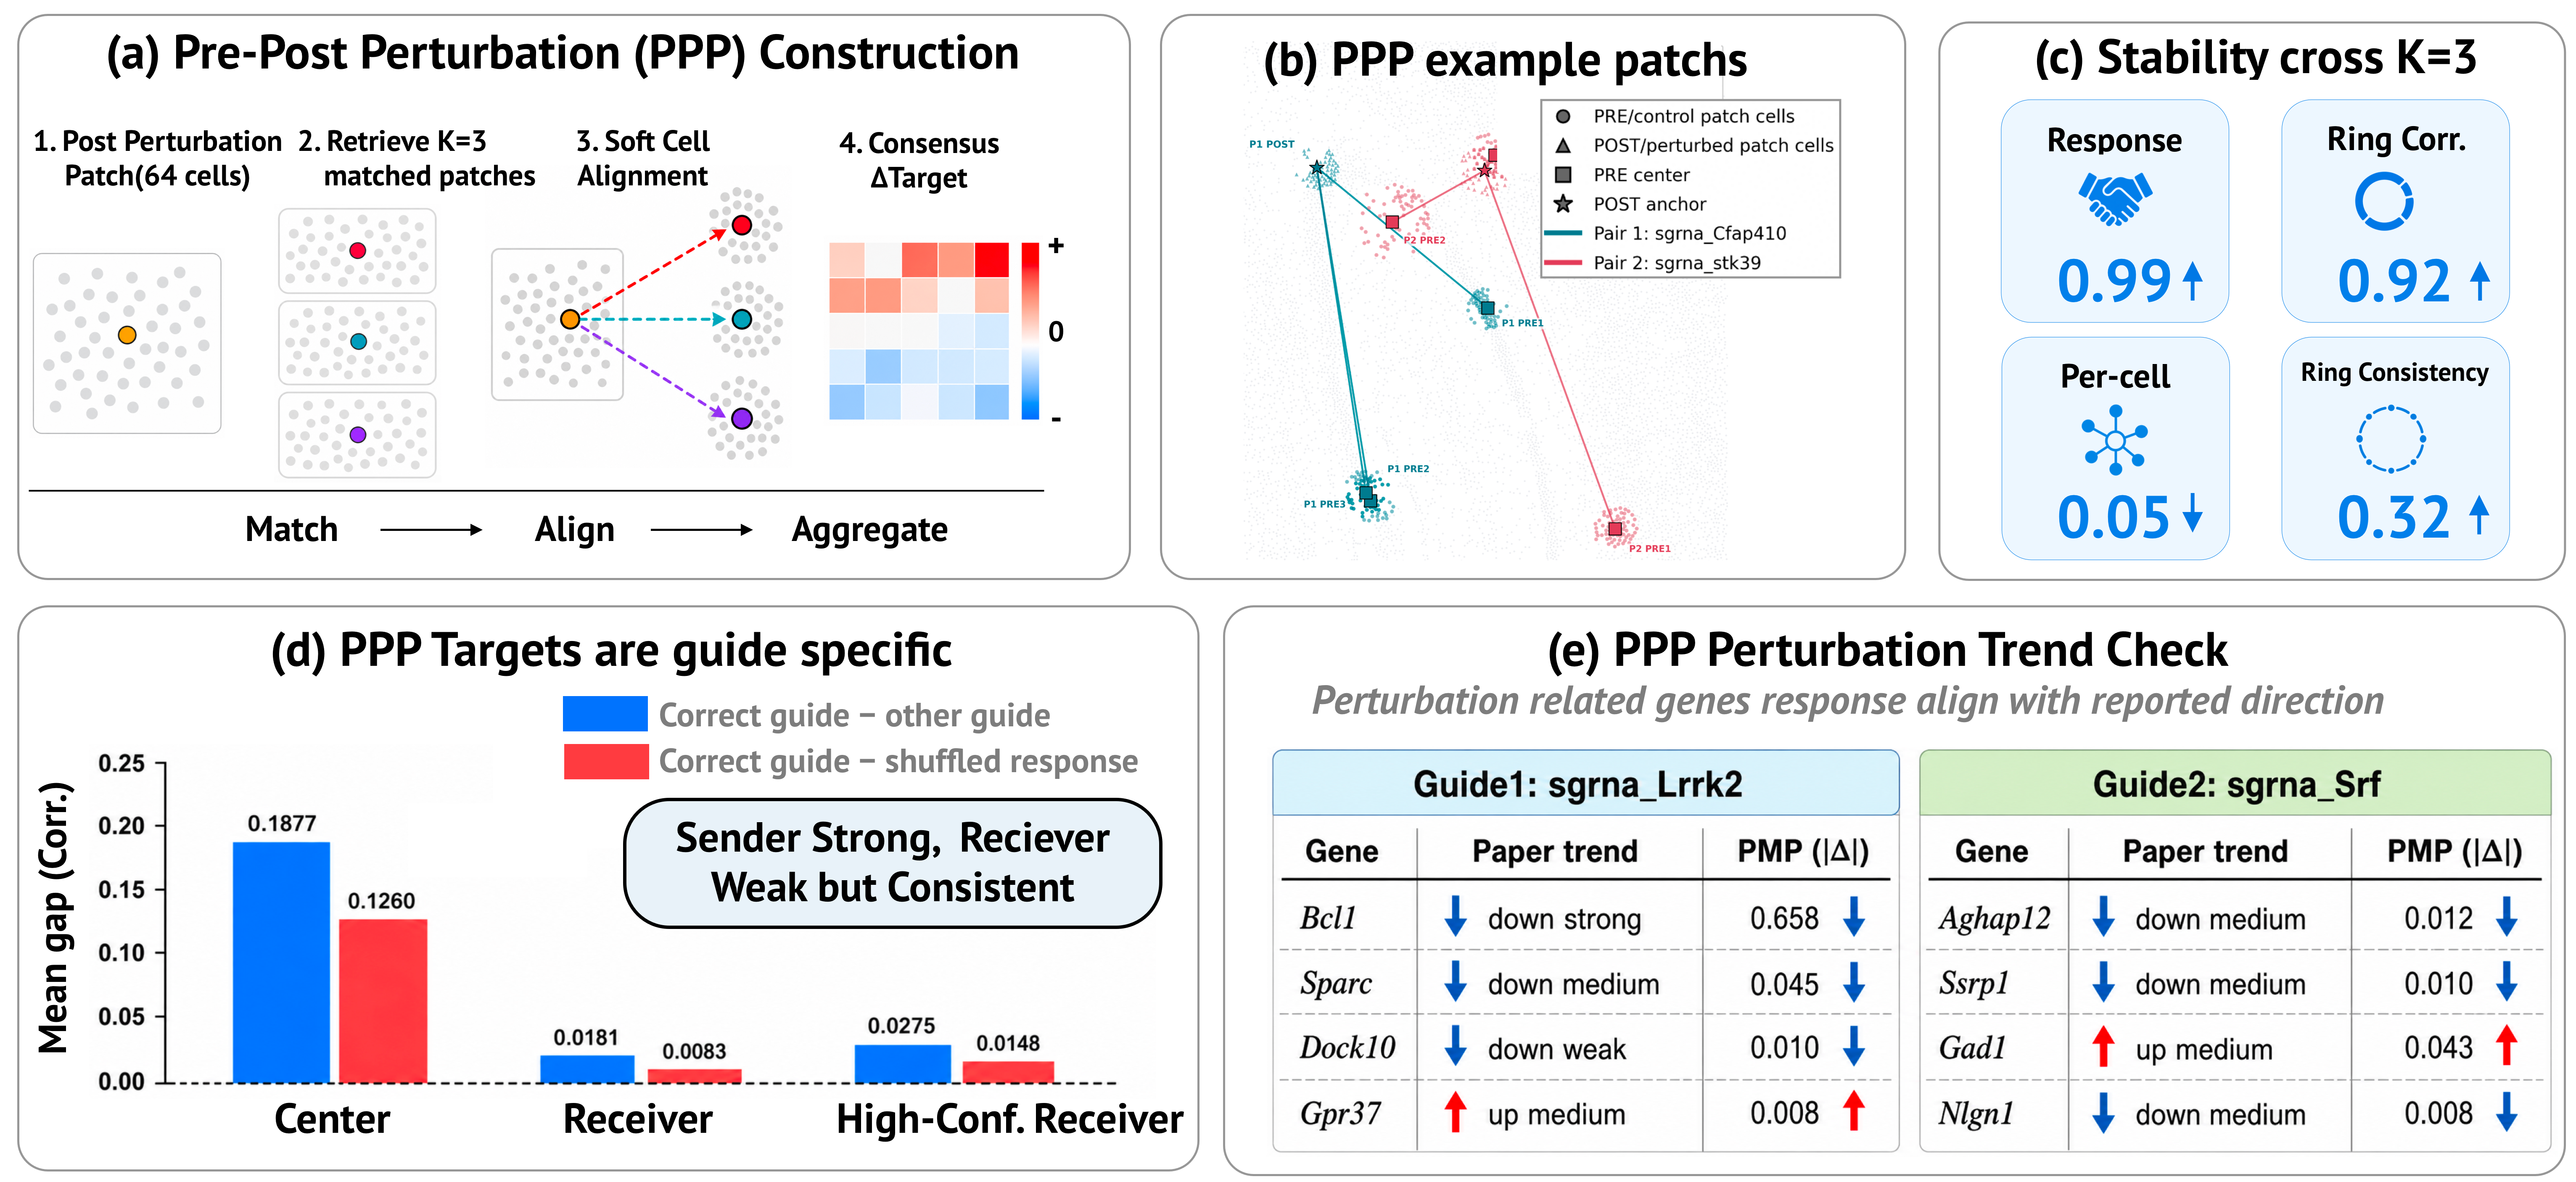
\includegraphics[width=0.9\linewidth]{pair_2.png}
\caption{\textbf{Pre-Post Perturbation Pairing(PPP) construction and validation.}
(a) Each post-perturbation 64-cell patch is matched to K=3 control patches, softly aligned, and aggregated into a consensus post–pre response target. (b) Example matched pre/post patches. (c–e) Stability and null audits show that PPP targets are consistent across matched controls and align more strongly with their own guide signatures than with wrong-guide or shuffled nulls. Full pseudocode and exact audit tables are provided in the supplementary material.}
\label{fig:data_pair}
\end{figure}
\subsection{Mining communication-rich ST micro-environments for propagation priors}
\label{sec:st_microenvironment_mining}
To enrich propagation priors, we mine response-like microenvironments from unperturbed mouse-brain reference ST. These regions provide program-enriched tissue neighborhoods for learning niche structure, cell--cell coupling, and communication-aware context. Specifically, we use two HD sections and three Xenium mouse-brain studies, mining seven response-like templates spanning interferon/inflammatory, microglial, astrocytic, myelin-lineage, neuronal, splicing, and mitochondrial/OXPHOS programs. Across 392{,}962 cells, this yields 1{,}619 positive reference anchors and 9{,}316 anchor--normal local pairs. These pairs pretrain the frozen organ-specific microenvironment encoder with gene-program, neighborhood, patch-composition, and communication-plausibility objectives, while signed response supervision remains defined by Spatial Perturb-seq (PPP) pairs. Detailed statistics are provided in the supplementary material.
\section{Method}
\label{sec:method}
\subsection{Model overview}
\label{sec:method_overview}
\paragraph{Task and graph interface.}
Given an unperturbed cell-resolved ST slide, a perturbation, and a set of direct-effect cells, \methodname{} predicts a signed response $\widehat\Delta_i$ for every cell in the local tissue graph. The cell-intrinsic response of direct-effect cells is provided as a direct-effect seed $d_i$, estimated from observed direct-effect-cell responses in measured Spatial Perturb-seq benchmarks or supplied by a trained single-cell perturbation model such as CPA in de novo inference. We instantiate this interface on local 64-cell directed graphs $P=(V,E)$. Each cell $i$ has matched-control expression $x_i\in\mathbb{R}^G$, cell state $c_i$, relative coordinate $p_i$, local geometry $g_i$, direct-effect indicator $a_i$, and direct-effect seed $d_i$ when $a_i=1$; neighbor cells have $a_i=0$ and $d_i=0$. Each directed edge $(i,j)$ carries spatial, cell-state-pair, and interaction-compatibility features $e_{ij}$, which act as soft routing information rather than causal communication labels.
\paragraph{Niche--propagation decomposition.}
\methodname{} is a perturbation-aware graph neural network that decomposes each cell-level PPP response target into niche impact and propagation impact:
\begin{equation}
\label{eq:niche_prop_decomposition}
\Delta_i = I_i^{\mathrm{niche}} + I_i^{\mathrm{prop}}, \qquad \widehat x_i^{\mathrm{post}} = x_i+\widehat\Delta_i .
\end{equation}
Here $I_i^{\mathrm{niche}}$ denotes the microenvironment-explainable component associated with baseline expression, local cell-state composition, tissue geometry, and niche context. $I_i^{\mathrm{prop}}$ denotes the remaining perturbation-associated component induced when direct-effect cells influence neighboring cells through the spatial graph. The model estimates these terms with a masked niche module, a direct-effect-to-neighbor propagation module, and a distance-aware refinement module.
\subsection{Niche impact estimation}
\label{sec:method_niche_impact}
\paragraph{Masked niche module.}
The niche module estimates the part of the response predictable from local tissue context alone. It is supervised against the cell-level PPP target $\Delta_i$, but direct-effect inputs are removed when the module is evaluated:
\begin{equation}
\label{eq:niche_module_target}
\widehat I_i^{\mathrm{niche}} = f_{\mathrm{niche}}(x,c,p,e;\,a=0,d=0), \qquad I_i^{\mathrm{prop},\star} = \Delta_i-\widehat I_i^{\mathrm{niche}} .
\end{equation}
The second term defines the propagation target. This prevents the propagation module from learning generic niche variation and forces it to focus on perturbation-associated spatial effects.
\subsection{Direct-effect-to-neighbor graph propagation}
\label{sec:method_graph_propagation}
\paragraph{State initialization.}
Each cell is embedded from matched-control and spatial features, then split into a neighbor state and a direct-effect state:
\begin{equation}
\label{eq:state_initialization}
h_i=\phi_x(x_i)+\phi_c(c_i)+\phi_p(p_i)+\phi_g(g_i), \qquad n_i^0=\phi_N(h_i), \qquad u_i^0=a_i\phi_D([h_i,d_i,g_i]) .
\end{equation}
The direct-effect state $u_i^0$ is nonzero only for direct-effect cells, so perturbation information enters the graph only through direct-effect cells.
\paragraph{Directed message passing.}
For direct-effect cell $i$ and neighbor cell $j$, the propagation module computes gated messages along graph edges and updates neighbor states:
\begin{equation}
\label{eq:directed_message_passing}
\begin{aligned}
\mu_{ij}^{\ell} &= \sigma\!\left(\phi_a([u_i^0,n_j^\ell,e_{ij}]) + w_{\mathrm{int}}q_{ij}\right)\phi_\mu([u_i^0,n_j^\ell,e_{ij}]),\\[-0.2em]
n_j^{\ell+1} &= \phi_u\!\left(\left[n_j^\ell,\,\sum_{i:(i,j)\in E,\,a_i=1}\mu_{ij}^{\ell}\right]\right).
\end{aligned}
\end{equation}
The compatibility score $q_{ij}$ biases routing but does not define a fixed communication graph. Direct-effect states are held fixed during propagation, and neighbor states are updated only by messages arriving through graph edges. The base propagation impact is decoded as
\begin{equation}
\label{eq:base_propagation_impact}
\widehat I_i^{\mathrm{prop},\mathrm{base}} = a_i\psi_{\mathrm{direct}}(u_i^0) + (1-a_i)\psi_{\mathrm{neighbor}}(n_i^L).
\end{equation}
\subsection{ST niche prior and distance-aware refinement}
\label{sec:method_st_refinement}
\paragraph{Reference-ST niche encoder.}
To improve generalization across tissue contexts, we pretrain a frozen niche encoder on large-scale unperturbed mouse-brain spatial transcriptomics. The encoder learns cell-level and patch-level microenvironment representations with self-supervised gene-program, neighborhood, patch-composition, and edge objectives. These representations provide perturbation-label-free niche priors for propagation, but are not treated as response labels or oracle communication edges.
\paragraph{Distance-aware refinement.}
After the first propagation pass, high-response neighbor cells are grouped into three distance rings around the direct-effect region: the nearest eight neighbors, the next 24 neighbors, and the remaining neighbors. Ring tokens summarize first-pass response structure and are injected into a second lightweight propagation pass, producing an ST-conditioned propagation impact $\widehat I_i^{\mathrm{prop},\mathrm{st}}$. The refinement is restricted to direct-effect cells and selected high-response neighbors, so it corrects spatially organized response patterns rather than uniformly rewriting the full patch. The final response is
\begin{equation}
\label{eq:final_response_prediction}
\widehat\Delta_i = \widehat I_i^{\mathrm{niche}} + (1-\alpha)\widehat I_i^{\mathrm{prop},\mathrm{base}} + \alpha\widehat I_i^{\mathrm{prop},\mathrm{st}}, \qquad \alpha=0.65 .
\end{equation}
All terms are response deltas; post-perturbation expression is reconstructed only after the final delta is predicted.
\subsection{Training and inference}
\label{sec:training_inference}
The reference-ST encoder and propagation model are trained with:
\begin{equation}
\label{eq:training_objectives}
\begin{aligned}
\mathcal{L}_{\mathrm{ref}} &= 2.0\mathcal{L}_{\mathrm{masked\text{-}program}} + 1.0\mathcal{L}_{\mathrm{neighborhood}} + 0.25\mathcal{L}_{\mathrm{patch\text{-}hist}} + 0.25\mathcal{L}_{\mathrm{edge}},\\[-0.2em]
\mathcal{L}_{\mathrm{prop}} &= 1.0\mathcal{L}_{\mathrm{neighbor}} + 0.3\mathcal{L}_{\mathrm{ring}} + 0.3\mathcal{L}_{\mathrm{post}} + 0.1\mathcal{L}_{\mathrm{rank}} .
\end{aligned}
\end{equation}
Training proceeds in four stages: reference-ST niche pretraining, niche-module training with perturbation inputs removed, propagation-module training on $I_i^{\mathrm{prop},\star}$, and distance-aware refinement with the frozen niche encoder attached through zero-initialized adapters. The direct-effect-cell loss is assigned zero weight in the strongest propagation setting so that neighbor-cell propagation is not dominated by the easier direct-effect prediction task. At inference time, the direct-effect seed is either computed from observed direct-effect-cell response or supplied by an external single-cell perturbation model, then propagated through the local tissue graph. Full equations and implementation details are provided in the supplementary material.
\section{Experiments}
\label{sec:experiments}
\subsection{Benchmark and metrics}
\label{sec:benchmark_metrics}
\textbf{Benchmark.}
We evaluate \methodname{} in three complementary settings: the mouse-brain Spatial Perturb-Seq benchmark in \Cref{sec:data_construction}, a controlled synthetic LR-propagation benchmark, and external Perturb-map validation. Together, they test cell-resolved neighbor prediction, recovery under known propagation rules, and agreement with coarser spatial CRISPR readouts. \textbf{Task and split.}
The primary Spatial Perturb-Seq task uses a 64-cell graph, direct-effect region, and direct-effect seed to predict the matched-control response field over direct-effect and neighbor cells; measured runs use observed seeds, while de novo runs use a single-cell predictor. We use two development slides and one held-out test slide, with no post anchor, matched-control patch, or 64-cell patch shared across partitions. The final split contains 2{,}179/2{,}179/928 train/validation/test patches, each with 512 genes, six cell types, and 23 edge features. \textbf{Metrics, baselines, and compute.}
We report Neighbor Pearson, centered/high-confidence variants, ring Pearson, Neighbor MAE, sender-center Pearson, plus synthetic LR and Perturb-map agreement. Baselines include statistical/retrieval, direct-effect/radial, supervised patch, and graph models; shortcut and input-ablation controls are reported separately. Unless noted, runs use 64-cell patches on one RTX A6000 via \texttt{--device cuda}; the organ/niche prior used an H100 GPU. Details are provided in the supplementary material.
\begin{figure}[t]
\centering
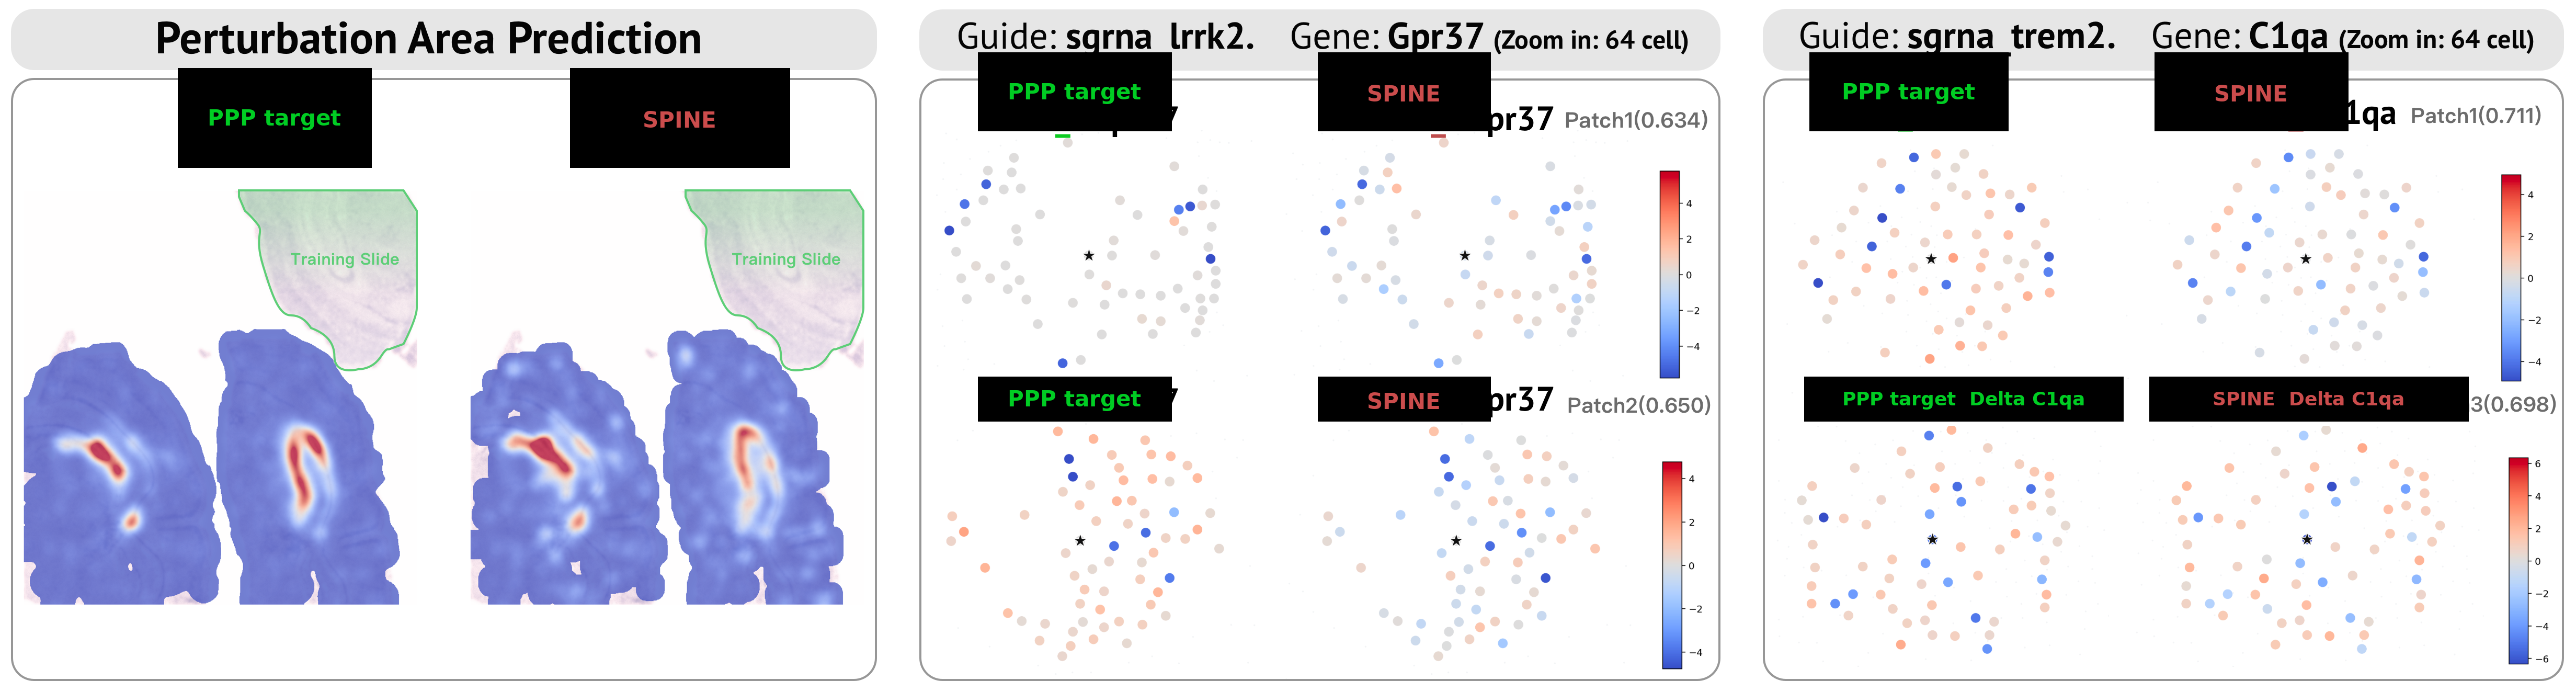
\includegraphics[width=0.90\linewidth]{main_exp.png}
\caption{\textbf{Main real-data evaluation on the Spatial Perturb-Seq mouse-brain benchmark.}
The visualization summarizes receiver-side perturbation prediction under the block-holdout matched-control setting, complementing the gene-centric quantitative analysis in \Cref{tab:main_results}. A full-resolution version with additional spatial and local-neighborhood panels is provided in the supplementary material.}
\label{fig:main_exp}
\end{figure}
% If not already defined:
% \newcommand{\pmv}[2]{#1\,{\scriptsize$\pm$}\,#2}
\begin{table*}[t]
\centering
\caption{\textbf{Validation across exact, controlled synthetic, and Spot level spatial perturbation datasets.}
(a) Gene-centric neighbor-cell performance on the exact cell-resolved Spatial Perturb-Seq benchmark.
(b) Controlled synthetic LR-propagation validation using external in vivo Perturb-seq direct-effect signatures.
(c) Spot/lesion-level external validation on Perturb-map.}
\label{tab:main_results}
\vspace{2pt}
\begin{minipage}[t]{0.585\linewidth}
\centering
\footnotesize
\setlength{\tabcolsep}{3.0pt}
\renewcommand{\arraystretch}{1.02}
\textbf{(a) Exact cell-resolved Spatial Perturb-Seq benchmark}
\vspace{2pt}
\resizebox{\linewidth}{!}{%
\begin{tabular}{@{}lcccc@{}}
\toprule
\textbf{Gene} &
\textbf{Mean $|\Delta|$} &
\textbf{Pearson} &
\textbf{$R^2$} &
\textbf{MAE} \\
\midrule
\rowcolor{gray!18}
\multicolumn{5}{@{}l}{\textbf{\textit{Perturbation-related genes.}}} \\
\textit{Gfap}   & \pmv{0.966}{0.016} & \pmv{0.788}{0.005} & \pmv{0.621}{0.007} & \pmv{0.785}{0.008} \\
\textit{Trem2}  & \pmv{0.324}{0.006} & \pmv{0.266}{0.005} & \pmv{0.047}{0.004} & \pmv{0.449}{0.005} \\
\textit{C1qa}   & \pmv{0.996}{0.012} & \pmv{0.835}{0.003} & \pmv{0.694}{0.005} & \pmv{0.690}{0.005} \\
\textit{Olig2}  & \pmv{0.287}{0.007} & \pmv{0.184}{0.006} & \pmv{0.018}{0.004} & \pmv{0.385}{0.005} \\
\textit{Opalin} & \pmv{0.868}{0.014} & \pmv{0.781}{0.003} & \pmv{0.601}{0.006} & \pmv{0.722}{0.006} \\
\midrule
\rowcolor{gray!18}
\multicolumn{5}{@{}l}{\textbf{\textit{Top five high-variance genes.}}} \\
\textit{Ptgds}  & \pmv{1.984}{0.010} & \pmv{0.805}{0.004} & \pmv{0.645}{0.007} & \pmv{1.087}{0.011} \\
\textit{Plp1}   & \pmv{1.743}{0.014} & \pmv{0.737}{0.005} & \pmv{0.533}{0.009} & \pmv{1.174}{0.013} \\
\textit{Ywhaz}  & \pmv{2.020}{0.010} & \pmv{0.772}{0.005} & \pmv{0.540}{0.011} & \pmv{1.274}{0.017} \\
\textit{Uqcrh}  & \pmv{1.971}{0.010} & \pmv{0.790}{0.004} & \pmv{0.616}{0.008} & \pmv{1.123}{0.012} \\
\textit{Sst}    & \pmv{2.031}{0.014} & \pmv{0.773}{0.006} & \pmv{0.580}{0.011} & \pmv{1.245}{0.019} \\
\midrule
\rowcolor{gray!18}
\multicolumn{5}{@{}l}{\textbf{\textit{High-change genes.}}} \\
\textit{Cycs}   & \pmv{2.356}{0.015} & \pmv{0.851}{0.003} & \pmv{0.708}{0.007} & \pmv{1.161}{0.014} \\
\textit{Nme2}   & \pmv{2.347}{0.014} & \pmv{0.874}{0.002} & \pmv{0.762}{0.004} & \pmv{1.051}{0.010} \\
\textit{Rack1}  & \pmv{2.333}{0.011} & \pmv{0.880}{0.002} & \pmv{0.759}{0.005} & \pmv{1.056}{0.011} \\
\textit{Ptma}   & \pmv{2.203}{0.012} & \pmv{0.882}{0.002} & \pmv{0.769}{0.004} & \pmv{1.008}{0.010} \\
\textit{Psmb4}  & \pmv{2.197}{0.008} & \pmv{0.826}{0.004} & \pmv{0.673}{0.007} & \pmv{1.132}{0.013} \\
\bottomrule
\end{tabular}
}
\end{minipage}
\hfill
\begin{minipage}[t]{0.392\linewidth}
\centering
\footnotesize
\setlength{\tabcolsep}{3.0pt}
\renewcommand{\arraystretch}{1.17}
\textbf{(b) synthetic LR-propagation validation}
\vspace{2pt}
\resizebox{\linewidth}{!}{%
\begin{tabular}{@{}lccc@{}}
\toprule
\textbf{Setting} &
\textbf{Recv. $r$} &
\textbf{Ring $r$} &
\textbf{$\Delta$Ring} \\
\midrule
Niche module only & 0.003 & 0.006 & -- \\
Synthetic fine-tuned & \textbf{0.619} & \textbf{0.815} & \textbf{0.809} \\
\midrule
Held-out perturbation & 0.274 & 0.550 & 0.541 \\
Held-out interface & 0.607 & 0.806 & 0.798 \\
Held-out strength $2.0$ & 0.520 & 0.807 & 0.798 \\
Held-out host patch & 0.597 & 0.806 & 0.801 \\
\bottomrule
\end{tabular}
}
\vspace{7pt}
\textbf{(c) Spot-level Perturb-map validation}
\vspace{2pt}
\resizebox{\linewidth}{!}{%
\begin{tabular}{@{}lccc@{}}
\toprule
\textbf{Readout} &
\textbf{Spot $r$} &
\textbf{95\% CI} &
\textbf{Lesion $\rho$} \\
\midrule
\textit{Ifngr2} top-25 & \textbf{0.853} & [0.811, 0.887] & 0.536 \\
\textit{Jak2} top-25   & \textbf{0.757} & [0.702, 0.801] & \textbf{0.929} \\
\textit{Tgfbr2} top-25 & \textbf{0.714} & [0.665, 0.755] & 0.607 \\
TGF$\beta$--stroma     & \textbf{0.808} & [0.765, 0.842] & 0.750 \\
IFN response            & 0.628 & -- & -- \\
\bottomrule
\end{tabular}
}
\vspace{2pt}
\parbox{\linewidth}{\scriptsize
For panel (c), spot-level Pearson values compare predicted and observed program scores after aggregation to Perturb-map spots.}
\end{minipage}
\vspace{-2pt}
\end{table*}
\subsection{Validation: Neighbor Responses Are Recovered Across Three Perturbation Datasets}
\label{sec:validation_main_benchmark}
We validate \methodname{} in three regimes: exact cell-resolved Spatial Perturb-Seq, controlled synthetic LR propagation, and spot/lesion-level Perturb-map validation. These settings test matched neighbor-cell prediction, learnability under known propagation rules, and cross-assay agreement under coarser spatial perturbation supervision.
\textbf{Cell-resolved Spatial Perturb-Seq validation.}
On the block-held-out Spatial Perturb-Seq test slide, \methodname{} reaches
neighbor-cell/ring Pearson $0.684/0.457$ with neighbor MAE $0.408$
(\Cref{fig:main_exp}; full gene-centric results are reported in the supplementary material). Gene-level recovery is strongest for
high-change receiver genes, with mean absolute delta above $2.19$ and Pearson
$0.826$--$0.882$; high-variance genes remain strong with Pearson
$0.737$--$0.805$; and perturbation-related genes are uneven but informative, with
\textit{C1qa}, \textit{Gfap}, and \textit{Opalin} recovered better than
\textit{Trem2} and \textit{Olig2}. Guide-stratified results show that the
aggregate is not driven by a few perturbations: across 14 test guides with at
least 20 patches, neighbor/ring Pearson is
$0.6851 \pm 0.0044$/$0.4604 \pm 0.0203$, with narrow per-guide ranges
($0.6767$--$0.6952$ and $0.4276$--$0.4956$). This is a stability audit of frozen
held-out predictions, not leave-one-guide-out retraining. Full guide-stratified
and aggregate gene-space metrics are reported in the supplementary material.
\textbf{Controlled synthetic LR-propagation validation.}
We next evaluate a synthetic benchmark combining external mouse in vivo
Perturb-seq direct-effect profiles from Jin \textit{et al.}, unperturbed
mouse-brain spatial graphs, and an LR-based receiver-response simulator. This is
not biological ground truth, but tests whether direct-effect-conditioned
propagation is learnable when the rule is known and tissue context alone should
not explain the target. Niche Module-only prediction is near zero
(neighbor/ring Pearson $0.003/0.006$), whereas synthetic fine-tuning recovers
held-out neighbor response fields with $0.619/0.815$. Performance remains strong
under held-out interface geometry, strength, and host-patch splits, and remains
non-trivial under held-out perturbations ($0.274/0.550$). Full analyses are in
\Cref{fig:synthetic_lr_summary,tab:synthetic_lr_main_models,tab:synthetic_lr_cross_split,tab:synthetic_lr_factor_breakdown,tab:synthetic_lr_mismatch_null}.
\textbf{Spot/lesion-level Perturb-map validation.}
Finally, we evaluate \methodname{} on Perturb-map / GSE193460, where perturbation
readouts are spot- or lesion-level rather than matched cell-resolved receiver
targets. We aggregate predicted response fields to gene programs and compare them
with observed spatial perturbation signatures. Predicted programs show strong
spot-level agreement for \textit{Ifngr2}, \textit{Jak2}, and \textit{Tgfbr2}
top-25 programs ($r=0.853$, $0.757$, and $0.714$), a curated
TGF$\beta$--stroma program ($r=0.808$), and an IFN-response program
($r=0.628$). Lesion-level ranking gives complementary support, with Spearman
correlations up to $0.929$ for \textit{Jak2} and $0.750$ for TGF$\beta$--stroma.
Bootstrap, top-$k$, and null-control analyses are reported in
\Cref{tab:perturbmap_external,tab:perturbmap_topk,tab:perturbmap_null_ci}.
\textbf{Strict grouped guide-out validation confirms perturbation-level generalization.}
In a strict grouped guide-out split, we jointly held out \textit{fasn}, \textit{stk39}, and \textit{trem2} from training and validation. On 992 unseen-guide graphs, \methodname{} achieved neighbor/ring Pearson $0.596/0.451$ with observed sender-side direct-effect seeds, outperforming elastic-net patch-summary regression $(0.334/0.142)$ and a Generic Graph Transformer without CCC priors $(0.497/0.395)$. Performance remained stable across all three held-out guides, showing that the result is not driven by one favorable perturbation and that the learned propagation module transfers to unseen guide identities. Full values are in \Cref{tab:strict_grouped_guide_out}.
\begin{table}[t]
\centering
\begin{minipage}[t]{0.49\linewidth}
\centering
\caption{Main benchmark against exact-task alternative models.}
\label{tab:main_baseline_comparison}
\scriptsize
\setlength{\tabcolsep}{2.5pt}
\renewcommand{\arraystretch}{1.00}
\resizebox{\linewidth}{!}{%
\begin{tabular}{lcccc}
\toprule
Baseline & Neighbor $\uparrow$ & Centered $\uparrow$ & Ring $\uparrow$ & MAE $\downarrow$ \\
\midrule
\rowcolor{gray!18}
\multicolumn{5}{l}{\textbf{\textit{Trivial, statistical, and retrieval baselines.}}} \\
Zero-delta & 0.000 & 0.000 & 0.000 & 0.453 \\
Guide$\times$type$\times$ring mean & 0.007 & -0.000 & 0.017 & 0.468 \\
Nearest patch transfer & 0.000 & -0.001 & 0.010 & 0.612 \\
\midrule
\rowcolor{gray!18}
\multicolumn{5}{l}{\textbf{\textit{Direct-effect and radial alternatives.}}} \\
Direct-effect diffusion & 0.006 & 0.000 & 0.014 & 0.459 \\
CCC-gated linear & -0.002 & 0.003 & 0.001 & 0.510 \\
Direct-effect broadcast & 0.016 & -0.000 & 0.053 & 0.835 \\
Direct-effect broadcast, fixed decay & 0.015 & 0.003 & 0.053 & 0.594 \\
Learned radial ridge & 0.023 & -0.002 & 0.066 & 0.527 \\
\midrule
\rowcolor{gray!18}
\multicolumn{5}{l}{\textbf{\textit{Supervised patch and graph alternatives.}}} \\
Elastic-net regression & 0.570 & 0.594 & 0.391 & 0.427 \\
Patch MLP & 0.272 & 0.444 & 0.087 & 0.677 \\
Graph Transformer patch model & 0.543 & 0.564 & 0.393 & 0.460 \\
Neural CCC-GNN & 0.543 & 0.565 & 0.393 & 0.464 \\
\midrule
\rowcolor{gray!18}
\multicolumn{5}{l}{\textbf{\textit{Niche--propagation model.}}} \\
\rowcolor{cyan!10}
\methodname{} final & \textbf{0.684} & \textbf{0.715} & \textbf{0.457} & \textbf{0.408} \\
\bottomrule
\end{tabular}%
}
\end{minipage}
\hfill
\begin{minipage}[t]{0.49\linewidth}
\centering
\caption{Input-effect and structural diagnostics on controlled synthetic and real benchmarks.}
\label{tab:seed_shortcut_controls}
\scriptsize
\setlength{\tabcolsep}{3pt}
\renewcommand{\arraystretch}{1.03}
\resizebox{\linewidth}{!}{%
\begin{tabular}{lccc}
\toprule
Diagnostic & Neighbor $\uparrow$ & Ring $\uparrow$ & Lift \\
\midrule
\rowcolor{gray!18}
\multicolumn{4}{l}{\textbf{\textit{Controlled synthetic LR ablation.}}} \\
Niche module only & 0.003 & 0.006 & \textemdash \\
Shuffle direct effect & 0.069 & 0.089 & $+0.000$ \\
Predicted direct effect & 0.611 & 0.803 & $+0.714$ \\
\rowcolor{cyan!10}
Final, measured direct effect & \textbf{0.619} & \textbf{0.815} & \textbf{$+0.726$} \\
\midrule
\rowcolor{gray!18}
\multicolumn{4}{l}{\textbf{\textit{Spatial Perturb-Seq ablation.}}} \\
Niche module only & 0.610 & 0.405 & \textemdash \\
Shuffle direct effect & 0.679 & 0.405 & $+0.000$ \\
Predicted direct effect & 0.680 & 0.417 & $+0.012$ \\
\rowcolor{cyan!10}
Final, measured direct effect & \textbf{0.684} & \textbf{0.457} & \textbf{$+0.052$} \\
\midrule
No niche-impact residualization & 0.165 & 0.153 & \textemdash \\
No edge attributes & 0.606 & 0.418 & $+0.013$ \\
No direct-effect input & 0.614 & 0.441 & $+0.036$ \\
\bottomrule
\end{tabular}%
}
\end{minipage}
\end{table}
\subsection{Ablations: Model Components and Direct-Effect Controls Add Complementary Evidence}
\label{sec:ablations}
\noindent\textbf{Input controls show that direct-effect seeds improve propagation beyond niche-only prediction.}
\Cref{tab:seed_shortcut_controls} evaluates direct-effect controls on both the controlled synthetic LR benchmark and the real Spatial Perturb-Seq benchmark. In the synthetic setting, the niche module alone is near zero, shuffled direct effects remain weak, and measured or predicted direct effects recover strong neighbor/ring performance ($0.619/0.815$ and $0.611/0.803$). In Spatial Perturb-Seq, measured direct effects provide the strongest real-data propagation signal, reaching $0.684/0.457$ and improving ring Pearson by $+0.052$ over the shuffled-seed control.
\noindent\textbf{Component ablations identify the structural sources of the gain.}
Removing niche-impact residualization causes the largest collapse, dropping neighbor/ring Pearson to $0.165/0.153$; this reflects both loss of niche-impact subtraction and the restricted direct-effect-to-neighbor routing of the propagation branch. Removing edge attributes weakens performance to $0.606/0.418$, and removing direct-effect input gives $0.614/0.441$, showing that spatial/communication features and perturbation-specific input provide complementary gains. Additional ablations are provided in the supplementary material.
\begin{figure}[t]
\centering
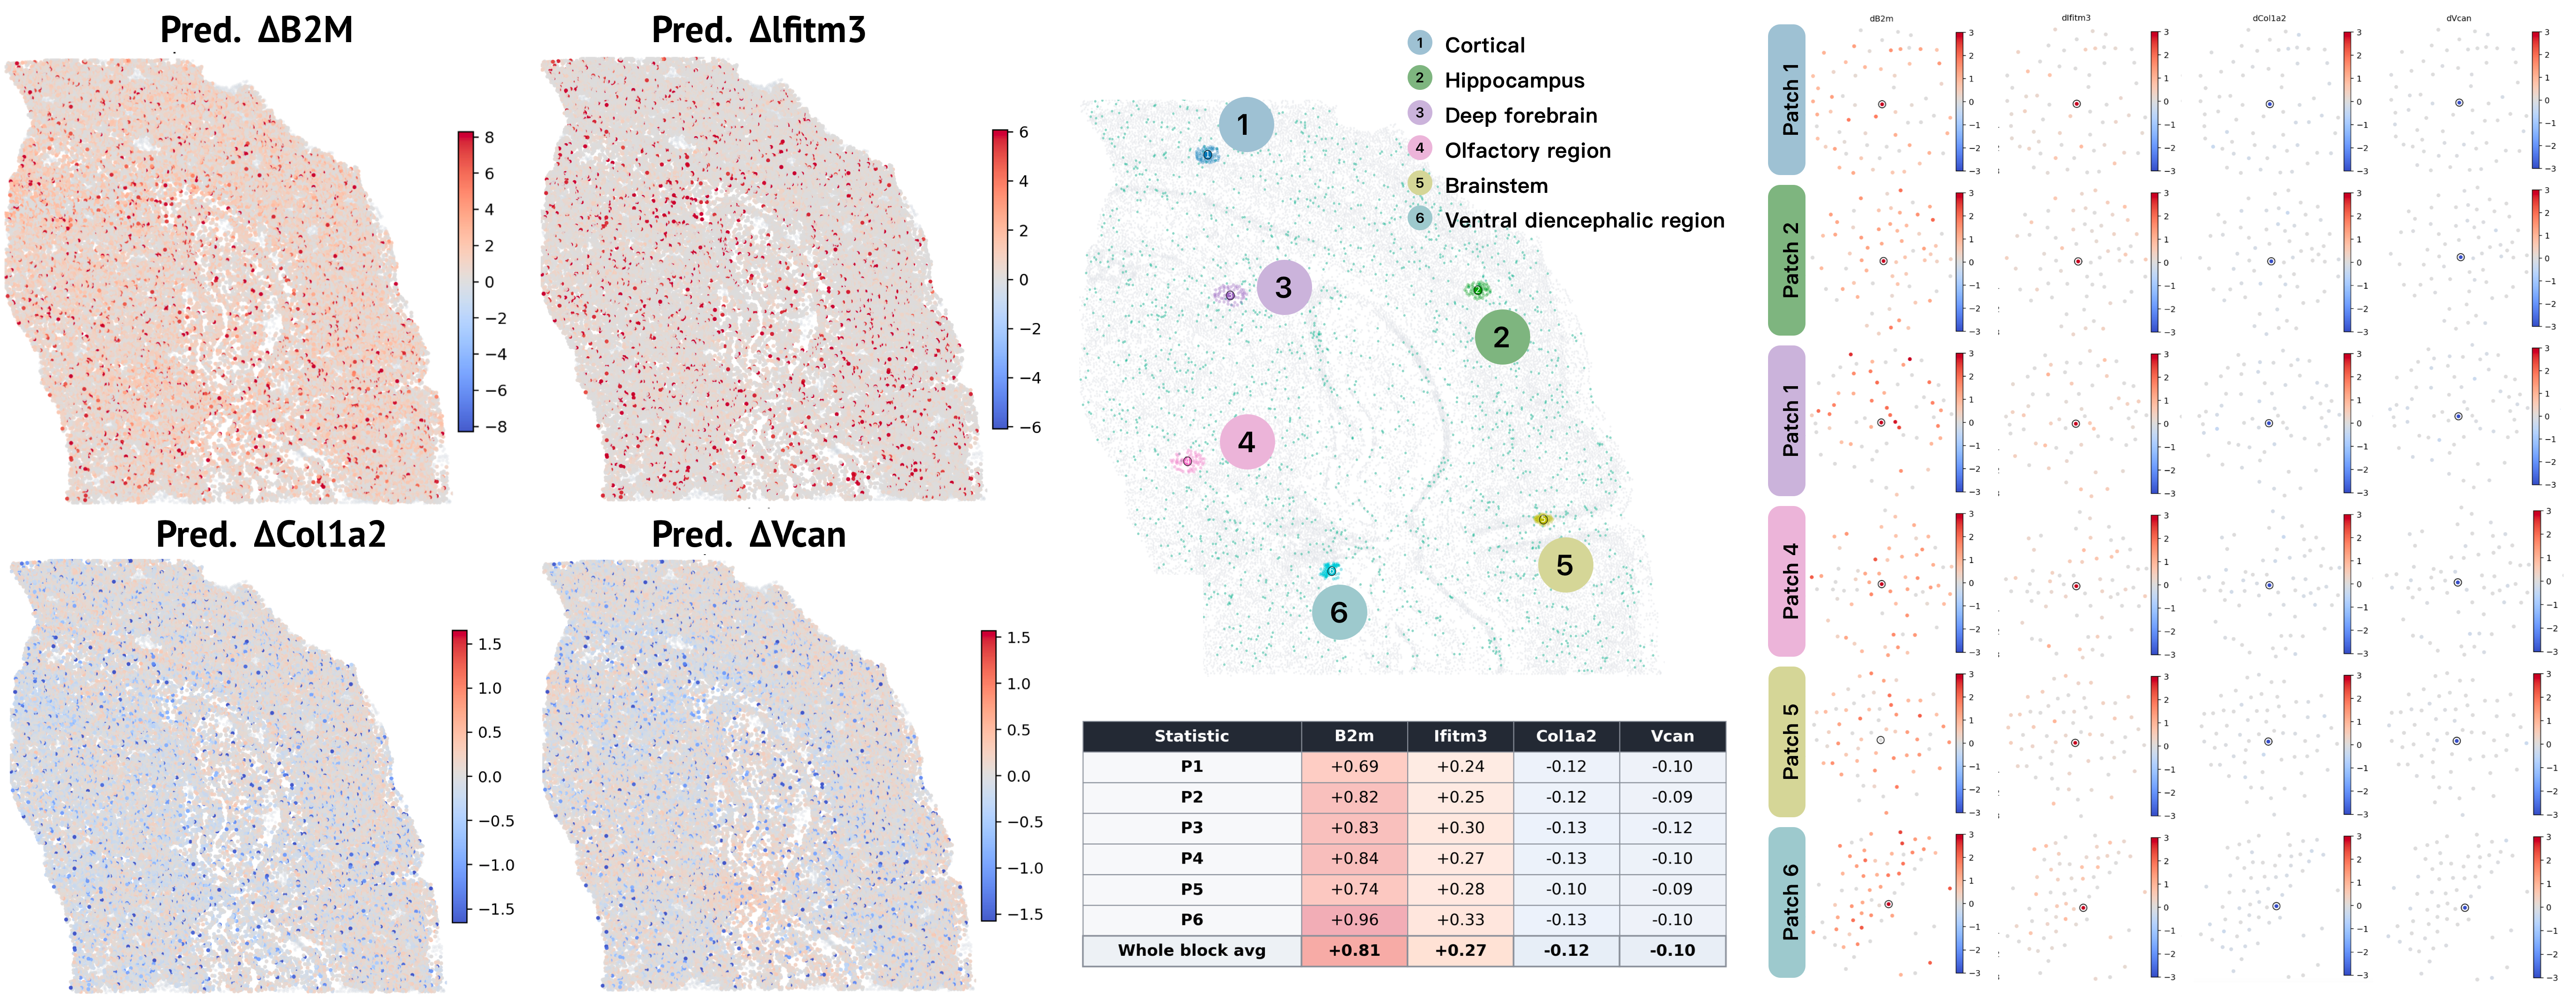
\includegraphics[width=\linewidth]{novo.png}
\caption{
\textbf{De novo IFN-$\gamma$ response-field prediction in mouse brain.}
Left: whole-tissue maps for representative IFN/MHC-I-associated and structural genes, showing positive \textit{B2m}/\textit{Ifitm3} and negative \textit{Col1a2}/\textit{Vcan} responses rather than a uniform shift.
Middle: six high-response regions with patch-averaged deltas overlaid on the spatial graph.
Right: local 64-cell neighborhoods, where highlighted target cells show the strongest response and nearby neighbors show structured propagation.}
\label{fig:ifng_response_field}
\end{figure}
\subsection{De novo IFN-\texorpdfstring{$\gamma$}{gamma} mouse-brain response-field case study}
\label{sec:ifng_case_study}
We use the trained propagation model as a de novo perturbation-query engine on an intact mouse-brain spatial graph. This setting has no paired IFN-$\gamma$ spatial perturbation labels. To construct the direct-effect seed, we train/fine-tune CPA on PerturbSapiens cytokine data, using treatment status (PBS/control versus IFN-$\gamma$), cell type, and tissue/broad class as covariates. For each Sample2/pre4 spatial cell, CPA predicts the IFN-$\gamma$ state and the matched control state; their difference gives a per-cell direct delta, which is then fed to the \methodname{} propagation module. This is a hypothesis-generation demonstration, not matched validation.
Figure~4 shows a heterogeneous response field across genes, regions, and local neighborhoods. \textbf{First, the model recovers the canonical IFN-$\gamma$/MHC-I program.} Target-cell deltas are positive for interferon and antigen-presentation genes, including \textit{B2m} $(+1.91)$, \textit{H2-D1} $(+1.57)$, and \textit{Ifitm3} $(+1.72)$, indicating a systematic IFN/MHC-I response across high-response targets. \textbf{Second, inferred IFN-$\gamma$ target cells are biased toward immune, vascular, and glial-associated states.} Microglia account for 11.91\% of top-pathway 5\% targets versus 7.98\% background frequency, a 1.49$\times$ enrichment. Endothelial and pericyte states are also mildly enriched, matching the expectation that IFN-$\gamma$ is sensed by immune, vascular, and glial microenvironments rather than arbitrary spatial locations. \textbf{Third, the perturbation is not only activating, it also suppresses structural and vascular-associated programs.} Target cells show down-regulation of \textit{Col1a2} $(-1.31)$, \textit{Vcan} $(-1.28)$, and \textit{Flt1} $(-1.82)$, suggesting a shift from homeostatic structural or vascular-like programs toward immune and antiviral programs. The response is spatially heterogeneous rather than a uniform slide shift: high-response patches show consistent IFN/MHC-I activation together with structural-gene suppression, and patch-level gradients reveal region-specific response direction and magnitude. Seed construction and full numerical readouts are reported in the supplementary material.
\section{Discussion, Limitations, and Conclusion}
\label{sec:discussion_limitations_conclusion}
Predicting perturbation responses inside intact tissue is needed for therapeutic
discovery, virtual tissue screening, and future virtual-patient modeling, where an
intervention can alter directly perturbed cells while also inducing secondary
responses in neighboring cells, local niches, and organ-scale programs.
\methodname{} addresses this missing spatial layer by modeling
direct-effect-to-neighbor propagation on cell-resolved tissue graphs, producing
spatial response-field predictions rather than isolated cell-autonomous outputs.  The central limitation is data availability: cell-resolved spatial perturbation
experiments are difficult to perform, and few public datasets support direct
evaluation in native tissue. We partially mitigate this by validating across an
exact Spatial Perturb-Seq benchmark, a controlled synthetic LR-propagation
benchmark, and real spot/lesion-level Perturb-map validation, with additional
Perturb-FISH sanity checks in the supplementary material. As more spatial perturbation datasets
appear across organs, disease contexts, and perturbation modalities, the same
framework can be trained and evaluated more broadly. 
Overall, \methodname{} turns single-cell direct-effect profiles into tissue-level
response-field hypotheses, providing a step toward spatially aware perturbation
modeling for experimental follow-up and intervention design.
\section{Code Release}
\label{sec:code_release}
We will release the anonymized code, configuration files, processed split manifests, benchmark construction scripts, and evaluation scripts in an \href{https://anonymous.4open.science/r/NICHETURB-F5E5/}{anonymous GitHub repository}.
\bibliographystyle{ACM-Reference-Format}
\bibliography{references}
\end{document}

